\documentclass{article}

\usepackage[a4paper, left=1.5cm, right=1.5cm, top=2cm, bottom=2cm]{geometry}

\usepackage{../../../../components/components}

\usepackage{hyperref}
\usepackage{fancyhdr}
\usepackage{listings}
\usepackage{tikz}
\usepackage{ccicons}
\usetikzlibrary{shapes.geometric, arrows.meta, positioning}

% Configuration des en-têtes et pieds de page
\pagestyle{fancy}
\fancyhf{} 

\fancyhead[L]{DL3 Math-Info PF5}
\fancyhead[C]{Programmation fonctionnelle}
\fancyhead[R]{2026-2027}

\fancyfoot[L]{Ewen Rodrigues de Oliveira\\\ccbyncsa}
\fancyfoot[R]{\thepage}

\begin{document}

\docTitle{Chapitre 7 : Compilation et architecture modulaire}

\section{Introduction à la compilation}

La \textbf{compilation} est la traduction d'un code source OCaml en un code exécutable cible (binaire machine ou code-octet). 

\remark{La compilation offre deux avantages par rapport à l'évaluation interactive (REPL) :
\begin{itemize}
    \item \textbf{Autonomie :} Génération d'un fichier exécutable autonome sans dépendance à l'environnement OCaml complet.
    \item \textbf{Efficacité :} Application d'optimisations statiques et vitesse d'exécution accrue.
\end{itemize}}

\subsection{Étapes de la compilation}

Le compilateur OCaml applique un traitement séquentiel structuré en plusieurs phases :

\begin{center}
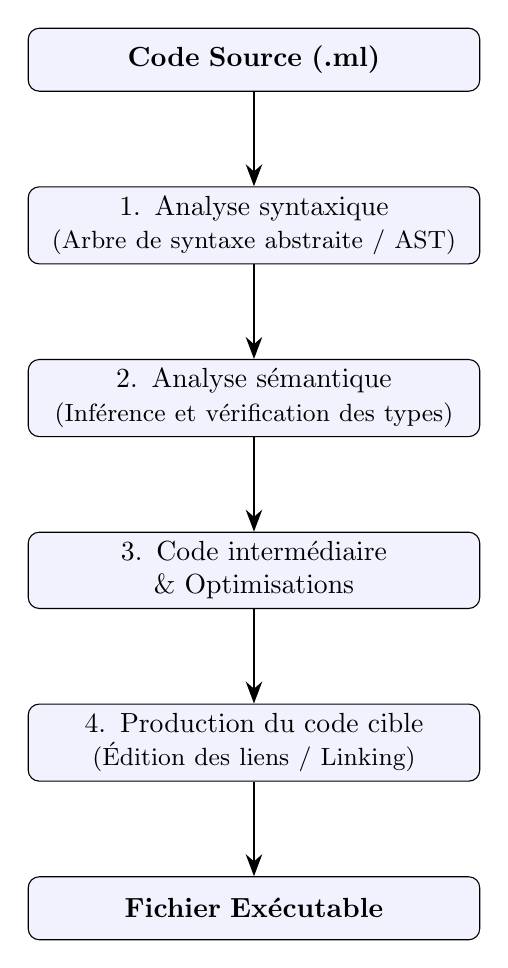
\begin{tikzpicture}[
    node distance=1.2cm,
    block/.style={rectangle, draw, fill=blue!5, text width=5.5cm, text centered, rounded corners, minimum height=0.8cm},
    line/.style={draw, -{Stealth[scale=1.2]}, thick}
]
    \node [block] (source) {\textbf{Code Source (.ml)}};
    \node [block, below=of source] (syntax) {1. Analyse syntaxique \\ \small(Arbre de syntaxe abstraite / AST)};
    \node [block, below=of syntax] (semantic) {2. Analyse sémantique \\ \small(Inférence et vérification des types)};
    \node [block, below=of semantic] (interm) {3. Code intermédiaire \& Optimisations};
    \node [block, below=of interm] (target) {4. Production du code cible \\ \small(Édition des liens / Linking)};
    \node [block, below=of target] (exec) {\textbf{Fichier Exécutable}};

    \path [line] (source) -- (syntax);
    \path [line] (syntax) -- (semantic);
    \path [line] (semantic) -- (interm);
    \path [line] (interm) -- (target);
    \path [line] (target) -- (exec);
\end{tikzpicture}
\end{center}

\subsection{Les deux formats de cibles d'OCaml}

\begin{enumerate}
    \item \textbf{Le code-octet (\textit{byte-code}) : } Compilateur \texttt{ocamlc}. Produit un code intermédiaire exécuté par la machine virtuelle OCaml. Fortement portable, temps de compilation minimal, mais exécution plus lente.
    \item \textbf{Le code natif : } Compilateur \texttt{ocamlopt}. Produit un binaire machine spécifique à l'architecture cible (x86, ARM, etc.). Performances optimales, exécutable totalement indépendant.
\end{enumerate}

\section{Interagir avec la ligne de commande : le module \texttt{Sys}}

Un exécutable compilé est évalué séquentiellement de haut en bas. L'interaction avec l'environnement s'effectue via les arguments passés au processus.

\method{Le tableau des arguments \texttt{Sys.argv}}{
    La valeur \texttt{Sys.argv}, de type \texttt{string array}, stocke les arguments de la ligne de commande :
    \begin{itemize}
        \item \texttt{Array.length Sys.argv} renvoie le nombre total d'arguments (nom du programme inclus).
        \item \texttt{Sys.argv.(0)} contient le nom ou le chemin de l'exécutable invoqué.
        \item \texttt{Sys.argv.(i)} (pour $i \ge 1$) contient le $i$-ème argument textuel.
    \end{itemize}
}

\example{Programme \texttt{argsimple.ml} d'affichage des arguments :}
\begin{lstlisting}[language=Caml]
let () =
  let nb_args = Array.length Sys.argv in
  for i = 0 to nb_args - 1 do
    Printf.printf "Argument numero %d : %s\n" i Sys.argv.(i)
  done
\end{lstlisting}

\noindent\textbf{Compilation et exécution dans le terminal :}
\begin{lstlisting}[language=bash]
$ ocamlc -o argsimple argsimple.ml
$ ./argsimple un deux trois
Argument numero 0 : ./argsimple
Argument numero 1 : un
Argument numero 2 : deux
Argument numero 3 : trois
\end{lstlisting}

\section{La programmation modulaire}

L'architecture d'un projet OCaml repose sur un découpage en unités logiques appelées \textbf{modules}.

\subsection{Architecture et graphe de dépendances}

Un module regroupe des définitions de types, de valeurs, de fonctions et d'exceptions. Les dépendances inter-modules doivent former un \textbf{graphe orienté acyclique} (DAG). Les dépendances cycliques sont interdites à la compilation.

\definition{Le module $A$ \textbf{dépend} du module $B$ si $A$ référence une entité exportée par l'interface de $B$.}

\begin{center}
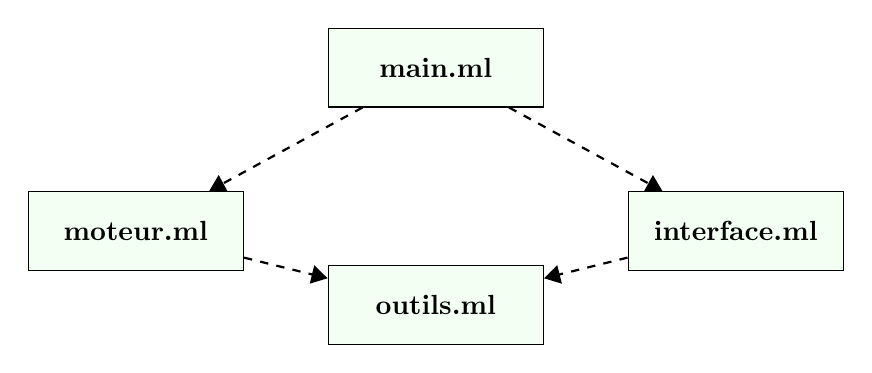
\begin{tikzpicture}[
    node distance=1.5cm,
    mod/.style={rectangle, draw, fill=green!5, text width=2.5cm, text centered, minimum height=1cm, font=\bfseries},
    dep/.style={draw, -{Triangle[scale=1.2]}, thick, dashed}
]
    \node [mod] (main) {main.ml};
    \node [mod, below left=of main] (m1) {moteur.ml};
    \node [mod, below right=of main] (ui) {interface.ml};
    \node [mod, below=2cm of main] (utils) {outils.ml};

    \path [dep] (main) -- (m1);
    \path [dep] (main) -- (ui);
    \path [dep] (m1) -- (utils);
    \path [dep] (ui) -- (utils);
\end{tikzpicture}
\end{center}

\subsection{Les Interfaces en OCaml (\texttt{.mli}) : Rôles et Utilisation}

Chaque module est scindé en deux composants : l'\textbf{implémentation} (\texttt{.ml}) et l'\textbf{interface} (\texttt{.mli}).

\subsubsection{Encapsulation et masquage}
L'interface agit comme un filtre d'accès. Toute entité définie dans le fichier \texttt{.ml} qui n'est pas explicitement déclarée dans le fichier \texttt{.mli} devient privée et inaccessible à l'extérieur du module.

\subsubsection{Abstraction des types}
Le fichier \texttt{.mli} permet de déclarer des \textbf{types abstraits}. En masquant l'implémentation concrète d'un type, on empêche l'extérieur de le manipuler directement ou d'effectuer du filtrage de motif dessus, garantissant l'invariance des données.

\example{Spécification abstraite (\texttt{tour.mli}) et implémentation concrète (\texttt{tour.ml}) :}

Fichier d'interface : \texttt{tour.mli}
\begin{lstlisting}[language=Caml]
type tower (* Type abstrait *)

exception Operation_illegal

val empty : tower
val push : int -> tower -> tower
val pop : tower -> tower
val top : tower -> int
\end{lstlisting}

Fichier d'implémentation : \texttt{tour.ml}
\begin{lstlisting}[language=Caml]
type tower = int list (* Structure de donnees concrete *)

exception Operation_illegal

let empty = []

let push x t = 
  match t with
  | [] -> [x]
  | h :: _ -> if x < h then x :: t else raise Operation_illegal

let pop t = 
  match t with
  | [] -> raise Operation_illegal
  | _ :: r -> r

let top t = 
  match t with
  | [] -> raise Operation_illegal
  | h :: _ -> h
\end{lstlisting}

\remark{L'abstraction de type assure le découplage : une modification de la structure interne dans le fichier \texttt{.ml} (par exemple remplacer une liste par un tableau) n'impacte aucunement les modules clients tant que le fichier \texttt{.mli} reste inchangé.}

\subsubsection{Ouverture de modules (\texttt{open})}
Par défaut, l'accès aux éléments d'un module s'effectue par nommage qualifié (ex: \texttt{Module.valeur}). La première lettre du nom du module est obligatoirement une majuscule.

\method{L'instruction \texttt{open}}{
    L'expression \texttt{open NomDuModule} importe l'ensemble du scope public du module dans l'environnement courant, dispensant de l'usage du préfixe qualificatif.
}

\example{Syntaxe d'importation dans \texttt{main.ml} :}
\begin{lstlisting}[language=Caml]
(* Approche 1 : Acces qualifie (Recommande pour la maintenance) *)
let pile1 = Tour.push 5 Tour.empty

(* Approche 2 : Ouverture globale du scope *)
open Tour
let pile2 = push 5 empty
\end{lstlisting}

\attention{L'ouverture globale via \texttt{open} peut induire des conflits de noms (masquage de fonctions homonymes). Il est recommandé d'utiliser des ouvertures locales restreintes : \texttt{let open Tour in push 5 empty} ou la syntaxe compacte \texttt{Tour.(push 5 empty)}.}

\subsection{Le mécanisme de compilation séparée}

La compilation séparée permet de compiler un module indépendamment de l'implémentation des modules dont il dépend : seule la connaissance de leurs interfaces est requise.

\method{Processus et extensions de fichiers}{
    Le compilateur génère des fichiers intermédiaires spécifiques :
    \begin{itemize}
        \item \texttt{ocamlc B.mli} $\rightarrow$ compile l'interface et génère le fichier binaire d'interface \texttt{B.cmi}.
        \item \texttt{ocamlc -c B.ml} $\rightarrow$ compile le corps du module (option \texttt{-c}, sans édition de liens) et génère le fichier objet \texttt{B.cmo} (\texttt{B.cmx} en code natif).
    \end{itemize}
    L'\textbf{édition des liens} rassemble les objets compilés pour produire l'exécutable : \\
    \texttt{ocamlc -o mon\_programme B.cmo A.cmo}.
}

\attention{L'ordre des fichiers objets lors du linking est strict : un module $B$ requis par un module $A$ doit impérativement précéder $A$ dans la commande de liaison.}

\section{Automatisation du build avec \texttt{make}}

L'outil \texttt{make} automatise la construction en résolvant le graphe de dépendances et en limitant la recompilation aux seuls fichiers modifiés ou impactés par une modification amont.

\example{\texttt{Makefile} générique pour le projet \texttt{tour} :}

\begin{lstlisting}[language=make]
# Regle principale : Edition des liens
main: tour.cmo main.cmo
	ocamlc -o main tour.cmo main.cmo

# Compilation de l'interface
tour.cmi: tour.mli
	ocamlc -c tour.mli

# Compilation de l'implementation (depend de sa propre interface)
tour.cmo: tour.cmi tour.ml
	ocamlc -c tour.ml

# Compilation du programme principal (depend de l'interface de Tour)
main.cmo: tour.cmi main.ml
	ocamlc -c main.ml

# Nettoyage des cibles intermédiaires
.PHONY: clean
clean:
	rm -f main *.cmi *.cmo
\end{lstlisting}

\newpage
\tableofcontents

\section*{Crédits}
Ce cours est mis à disposition selon les termes de la Licence Creative Commons \ccbyncsa\ \textbf{Attribution - Pas d'Utilisation Commerciale - Partage dans les Mêmes Conditions 4.0 International}. 
Pour voir une copie de cette licence, visitez \url{http://creativecommons.org/licenses/by-nc-sa/4.0/}.

\end{document}